\subsection{Benachrichtigung des Benutzers}\label{ss:benachrichtigung}

Mit der Verbreitung von Smartphones und mobilem Internet sind wie immer und überall erreichbar. Doch wir wüssten auch gerne was bei uns zu Hause passiert. Aus diesem Grund soll das Überwachungssystem im Falle eines Einbruchs den Besitzer alarmieren. Dies kann über eine Vielzahl von Möglichkeiten geschehen. 


\begin{table}[H] 
	\centering
	\begin{tabular}{|r||c|c|}\hline
		Informationskanal & Unverzögert & Übertragung von Medien\\ \hline \hline
		SMS & Ja & Nein \\ \hline
		Email & Nein & Ja \\ \hline
		Push-Notifications & Ja & Nein \\ \hline
	\end{tabular}
	\caption{Auflistung der mobil abrufbaren Kommunikationskanäle}
	\label{t:benachrichtugung}
\end{table}

Die klassische Email ist ein Kommunikationskanal, der auch unterwegs abgerufen werden kann. Der Nachteil hiervon ist jedoch, dass das Abrufen meist Zeitverzögert stattfindet und ein reagieren auf eine Einbruchsmeldung möglicherweise zu spät stattfindet. Sie bietet jedoch einige Vorteile: Man kann sie beinahe überall abrufen, da die Email ein universelles Kommunikationsmittel ist. Zudem können sowohl Text als auch Bilder oder Videos in einer Email verschickt werden. 

Die SMS ist im Vergleich zur Email unverzögert.  Direkt nach dem Eintreten des Unfalls wird der Benutzer informiert und kann reagieren. Leider können in einer SMS keine Bilder oder Videos übertragen werden, weshalb sie nicht das volle potential eines Smartphones ausschöpft.

Die Push-Benachrichtigung ist ein zentraler applikationsübergreifender Kommunikationskanal mobiler Geräte. Dabei wird die Kommunikation nicht vom Client (Smartphone / Tablet) initiiert, sondern von einem Server des Herstellers. Auf diese Weise ist es möglich, dem Besitzer des Sicherheitssystems ohne sein Zutun eine Nachricht zu übermitteln. Diese kann einen Text oder Link enthalten.\\
Durch die Verwendung von Push-Benachrichtigungen kann das Smartphone des Besitzers angewiesen werden eine App des Sicherheitssystems zu öffnen und die aktuellen Meldungen anzuzeigen. Ebenfalls ist es denkbar, dass der Benutzer nach dem Empfang der Push-Benachrichtigung automatisch eine vom Sicherheitssystem erstellte Webseite öffnet, auf der er Bilder oder Videos des Einbruchs ansehen kann.


\begin{figure}[H] 
	\centering
	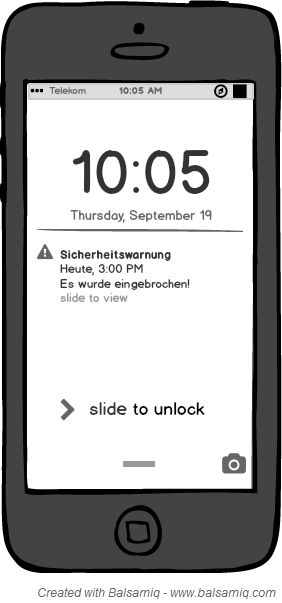
\includegraphics[scale=0.5]{Bilder/alert}
	\caption{Mockup einer Push-Benarichtigung}
	\label{f:alert}
\end{figure}
\todo[inline]{"Created with" herausnehmen}
